\documentclass[11pt,a4paper]{article}
\usepackage[utf8]{inputenc}
\usepackage[T1]{fontenc}
\usepackage{amsmath}
\usepackage{amssymb}
\usepackage{graphicx}
\usepackage[left=20mm, right=20.00mm, top=20.00mm, bottom=15.00mm]{geometry}
\usepackage{amsthm}
\usepackage{enumitem}
\usepackage{bm}
\usepackage{listings}
\usepackage{xcolor}
\usepackage{algpseudocode}
\usepackage{hyperref}



\theoremstyle{definition}
\newtheorem{definition}{Definition}[section]


\definecolor{codegreen}{rgb}{0,0.6,0}
\definecolor{codegray}{rgb}{0.5,0.5,0.5}
\definecolor{codepurple}{rgb}{0.58,0,0.82}
\definecolor{backcolour}{rgb}{0.95,0.95,0.92}

\lstdefinestyle{mystyle}{
	backgroundcolor=\color{backcolour},   
	commentstyle=\color{codegreen},
	keywordstyle=\color{magenta},
	numberstyle=\tiny\color{codegray},
	stringstyle=\color{codepurple},
	basicstyle=\ttfamily\footnotesize,
	breakatwhitespace=false,         
	breaklines=true,                 
	captionpos=b,                    
	keepspaces=true,                 
	numbers=left,                    
	numbersep=5pt,                  
	showspaces=false,                
	showstringspaces=false,
	showtabs=false,                  
	tabsize=2
}

\lstset{style=mystyle}

\begin{document}
	\begin{titlepage}
		\begin{minipage}{.10\textwidth}
			
\includegraphics[width=\textwidth]{images/left_logo.png}
		\end{minipage}%
		\begin{minipage}{.80\textwidth}
			\centering
			\Large
			\textbf{MIDDLE EAST TECHNICAL UNIVERSITY \\DEPARTMENT OF COMPUTER ENGINEERING}
		\end{minipage}%
		\begin{minipage}{.10\textwidth}
			
\includegraphics[width=\textwidth]{images/right_logo.png}
		\end{minipage}% 
		\vspace{2cm}
		
		\begin{center}
			\huge
			\textbf{SUMMER PRACTICE REPORT \\ CENG 400 \\}
			\vspace{2cm}
		\end{center}
	
		\large
		\begingroup
		\renewcommand{\arraystretch}{2.0} % Default value: 1
		\begin{tabular}{ p{5.6cm} p{10cm} }
			\textbf{STUDENT NAME} & Sait Elmas \\
			\textbf{ORGANIZATION NAME} & METU Computer Engineering Department Parallel Processing Laboratory \\
			\textbf{ADRESS} & Dept. of Computer Engineering Middle East Technical University Inonu Bulvari, 06531 Ankara, TURKEY \\
			\textbf{START DATE} & 1 August 2022 \\
			\textbf{END DATE} & 12 September 2022\\
			\textbf{TOTAL WORKING DAYS} & 30 days \\
		\end{tabular}
		\vspace{2cm}
		\endgroup

		\begin{tabular}{p{9cm} p{9cm}}
			\textbf{STUDENT'S SIGNATURE} & \textbf{ORGANIZATION APPROVAL} \\
		\end{tabular}
		
	\end{titlepage}
	
	\tableofcontents
	\newpage
	
	\section{Introduction}
		In the summer practice period I worked in the \textbf{Parallel Processing Laboratory} of Middle East Technical University, Computer Engineering Department. Active research areas are listed on the web page of laboratory as:
		\begin{itemize}
			\item High Performance Computing
			\item Development of parallel algorithms and their applications in science and engineering
			\item Parallel sparse matrix computations
			\item Parallel application development and run-time environments
		\end{itemize}
		Beside these research areas there are courses that are being lectured by the members of laboratory to the undergraduate/graduate level students. Some of the courses are:
		\begin{itemize}
			\item CENG371 – Scientific Computing
			\item CENG478 – Introduction to Parallel Computing
			\item CENG487 – Introduction to Quantum Computing
			\item CENG571 – Numerical Analysis
			\item CENG577 – Parallel Computing
			\item CENG780 – Sparse Matrix Computations
		\end{itemize}
		
		After my application for summer practice internship and undergraduate student researcher positions, \textbf{Prof. Murat Manguoğlu} has offered the topic of "random sparse matrix factorization".
		
		A matrix (array) that contains "a lot of" zeros is called a \textbf{sparse matrix (array)}. Although the ratio of zeros to the non-zeros is not strictly defined for a sparse matrix it will not be wrong to say that for a large matrix if the number of zeros are equal to the number of columns or rows that it is a sparse matrix. 
		
		In scientific computations the deterministic matrix algorithms are lack to solve the problems containing sparse matrices. One reason of that is these large matrices containing mostly zeros require many floating point operations that will easily overwhelming the capacity of even very powerful workstations.  Another reason of this challenge is large matrices takes so much space to fit in the primary memory so there will be need more that one passes to gain the information from the disc and after the application of the relevant algorithm writing it to the disk back. In this situation the performance is measured by the amount of disk access.
		
		For the first problem mentioned above "random methods" are in use. The idea is to sample the given matrix in such a way that the relatively simple sample contains \textit{nearly} all information of the sparse matrix. That is it spans nearly same linear space with the original sparse matrix space. With this simple representative deterministic matrix methods of software packets can be utilized. For the second problem "parallel processing" algorithms are mainly in focus. This topic has not been studied under this summer practice period.
		
	\section{Information About Project}
	
	As mentioned in the introduction section "random methods for sparse matrix factorization" has been studied as a solution of the first major problem of sparse matrix computations. I had worked on this method by applying the algorithms that are defined in the article \textbf{"Finding Structure with Randomness: Probabilistic Algorithms for Constructing Approximate Matrix Decompositions"} by \textbf{N. Halko, P. G. Martinson, J. A. Tropp}. For the applications the \textbf{"Julia Language"} utilized.
	
	The progress of this work has been supervised by Prof. Murat Manguoğlu via periodical meetings. 
	
	\subsection{Analysis Phase}
	At this stage a review of basic linear algebra, an introductory course about numberical linear algebra and tutorials for julia-language has been studied.		

	\subsubsection{Basic Linear Algebra}
	In this part some preliminary linear algebra subjects are listed. Although they are very basic it may be desirable to see all the terms that will be used at this report in one place. \\
	This part is heavily depend on the book \textit{\textbf{Linear Algebra} by \textbf{Stephan H. Friedberg}} and some related \textbf{wikipedia} pages.
	\begin{definition}[Vector Space]
		A \textbf{vector space} $V$ over a field $F$ (we mainly work with the fields of real and complex numbers ($\mathbb{R},\mathbb{C})$, so no need to define what a field is!) consist of two sets V (set of vectors), F (the field) and two operations + (addition) and $\cdot $ (scalar multiplication). Addition is defined on the set $V$ that is we want to add the vectors to each other. And scalar multiplication is the relation between vectors and the field $\mathbb{R}$ or $\mathbb{C}$, all together with the following properties: \\
		For any vector $v, v_1, v_2, v_3$ in $V$ and for any number $a,b$ in $\mathbb{R}$ 
		\begin{itemize}
			\item \textbf{Commutative} vector addition: $v_1 + v_2 = v_2 + v_1$
			\item \textbf{Associative} vector addition: $v_1 + (v_2 + v_3) = (v_1 + v_2) + v_3$
			\item There must be a \textbf{0 element} satisfying: $0+v = v+0 = v$
			\item Every vector $v$ should have an \textbf{inverse} $e$ such that $ v+e = 0$
			\item $1v = v1 = v$
			\item $(ab)v = a(bv)$
			\item $(a+b)v_1 = av_1 + av_2 $
			\item $a(v_1 + v_2) = av_1 + av_2$
		\end{itemize}
	$ \mathbb{R}^n$ is an example for a vector space over $\mathbb{R}$. $(1,2,3) + (2,3,4) = (2,3,4) + (1,2,3)$ for the vectors in $\mathbb{R}^3$ for instance and $(2*3)\cdot(1,2,3,4) = 2\cdot(3,6,9,12)$ in $\mathbb{R}^4$. All the properties can be easily verified for this natural vector space. \\
	An other basic example is the set of all complex valued $mxn$ dimensional matrices overt the field of complex numbers $\mathbb{C}$
	\end{definition}
	\begin{definition}[Inner Product]
		Let $V$ be a vector space over a field ($\mathbb{R}$ or $\mathbb{C}$). An \textbf{inner product} on $V$ is a function that takes two vectors and gives a number from the field. It is usually denoted as $\langle x,y \rangle$ or just $ x \cdot y$ with the following properties hold:
		\begin{enumerate}[label=(\alph*)]
			\item $\langle x + z, y \rangle = \langle x, y \rangle + \langle z,y \rangle $
			\item $\langle cx,y \rangle = c \langle x,y \rangle$
			\item $\overline{\langle x,y \rangle} = \langle y,x \rangle$. here the bar represents the complex conjugate of the number. If the field is the real numbers than it can be ignored.
			\item $ \langle x,x \rangle > 0$ if $x \neq 0$
		\end{enumerate}
 	\end{definition}
	An example of inner product is the standard Hermitian product on $\mathbb{C}^n$ as: $$ \langle \bm{x,y} \rangle = \sum_{j=1}^{n}x_j\bar y_j \text{ where } \bm{x} = (x_1, x_2, ... x_n), \bm{y}= (y_1, y_2, ... , y_n)$$
	
	\begin{definition}[Inner Product Space]
		A vector space over a field equipped with an inner product is called an \textbf{inner product space}
	\end{definition}
	
	\begin{definition}[Norm] Let $V$ be a vector space over real or complex numbers.  \textbf{Norm} of a vector is a function that assigns a real number to every vector in the vector space. It is denoted as $ \left\| \bm{x} \right\|$. The function should satisfy following three properties.
		\begin{enumerate}
			\item \textbf{Triangle inequality}: $ \left\| \bm{x+y}\right\| \leq \left\|\bm{x}\right\| + \left\| \bm{y}\right\|$
			\item $\left\| r\bm{x}\right\| = |r|\left\| \bm{x}\right\|$
			\item $ \left\|\bm{x}\right\| \geq 0 $ for any $\bm{x}$ and  $ \left\|\bm{x}\right\| = 0 $ if and only if $ \bm{x} = 0$
		\end{enumerate}
	\end{definition}
	
	
	In different sources norms are denoted in different symbols and even with different names so it may be confusing while reading technical documents. Here is a list of basic norms with their definitions. For $\bm{x} = (x_1, x_2, ... , x_n) \in \mathbb{R}^n$
	\begin{itemize}
		\item $\bm{l_1}$ \textbf{norm} (\textit{Taxicap norm, Manhattan norm}): $\left\| \bm{x}\right\|_1 = \sum_{j=1}^{n} |x_j| $ 
		\item $\bm{l_2}$ \textbf{norm}: $\left\| \bm{x}\right\|_2 = \sqrt{\sum_{j=1}^{n} |x_j|^2} $. This is the standart \textbf{Euclidian Distance}. With $l_2$ norm and standart inner product of vectors of $\mathbb{R}^n$ has the canonical relation as $ \left\| \bm{x}\right\|_2 = \sqrt{ \langle \bm{x,x} \rangle }$
		\item $\bf{l_p}$ \textbf{norm} ($p$ norm): $\left\| \bm{x}\right\|_p = \left( \sum_{j=1}^{n} |x_j|^2 \right)^{1/p} $
		\item $\bm{l_{\infty}}$ \textbf{norm} \textit{(Infinity norm, maximum norm)} $\left\| \bm{x}\right\|_{\infty} = \underset{i}{max} |x_i| $
	\end{itemize}

	\begin{definition}
		For an inner product space $V$ if the product of two vectors $\bm{x}$ and $bm{y}$, $\langle \bm{x,y} \rangle = 0$ than we say that $\bm{x}$ and $\bm{y}$ are \textbf{orthogonal} (perpendicular) to each other. If length of a vector is 1 that is $ \left\|\bf{x} \right\|_2 = 1 $ than we call it \textbf{unit vector}. If a set of vectors are mutually orthogonal to each other this set is called orthogonal. Additionally an orthogonal set with every vector has length 1 is called \textbf{orthonormal} set. \\
		All of these terms can be extended to define matrices with its columns are regarded as column vectors. A matrix is called orthogonal if all of its columns are mutually perpendicular and orthonormal if length of each column vector is 1 and they are orthogonal.
	\end{definition}

	\begin{definition}[Rank of a matrix]
		The \textbf{rank of a matrix} is the number of its columns that are linearly independent.
	\end{definition}
	\begin{definition}[Orthogonalization]
		Orthogonalization of a matrix A is finding a matrix say Q, that is orthonormal and that can span the same space with A. Q has rank(A) number of columns.
	\end{definition}
	In Matlab the \texttt{orth} command draws an orthonormal matrix for a given matrix A. As a simple function that computes the orthonormal matrix Q for a given matrix can be scripted as below. The method behind this function is called \textbf{Gram-Schmidt} orthogonalization process.
	
	\begin{definition}[Unitary Matrix]
		A square matrix $A$ is called \textbf{unitary} if $AA^H = A^HA = I$ where $A+H$ denotes the \textbf{conjugate transpose} of $A$.
	\end{definition}
	\begin{definition}[Normal Matrix]
		A square matrix $A$ is called \textbf{normal} if $AA^H = A^HA$.
	\end{definition}
	\begin{definition}[Hermitian Matrix]
		A square matrix $A$ is called \textbf{Hermitian} if $A = A^H$.
	\end{definition}
	\subsubsection{Matrix Factorization}
	Writing a matrix as a product of two relatively "simple" matrices may simplify complicated and expensive calculations. Here are some basic matrix factorizations. 
	\paragraph{Eigendecomposition}
	If a square matrix $A$ is diagonalizable than it can be written as $A=QDQ^{-1}$ where $Q$ contains eigenvectors as its columns and $D$ is a diagonal matrix containing the eigenvectors of A on the diagonal entries. One of the important properties of this decomposition is powers of the matrix $A$ can be calculated as:
	$$ A^n = (QVQ^{-1})^n = QVQ^{-1}QVQ^{-1} ... QVQ^{-1}QVQ^{-1} = QV^nQ^{-1} $$
	Evaluating powers of a diagonal matrix is very easy for both human and computer.
	\paragraph{QR Decomposition}
	Writing a matrix $A$ as a product of two matrices as $A= QR$ , where $Q$ is orthogonal and $R$ is upper triangular.
	\paragraph{Singular Value Decomposition}
	For a $m\times n$ matrix $A$ the SVD is the product of three matrices as $A = U\Sigma V^* $. Here $U$ is $m \times m$ complex unitary matrix, $V$ is $n \times n$ complex unitary matrix and $\Sigma$ is $m \times n$ rectangular diagonal matrix. 
	$$ \underset{m \times n}{A} = \underset{m \times m}{Q}\cdot \underset{m \times n}{\Sigma}\cdot \underset{n \times n}{V^*}$$
	
	The diagonal entries $\sigma_i = (\Sigma)_{ii}$ are called singular values of $A$. They are uniquely determined by the matrix $A$. They are spaced on the diagonal in descending order..
	\subsubsection{Matrix Norms (Operator Norms)}
	\begin{definition}[Matrix Norm]
		If we see the set of all $m \times n$ matrices with real of complex entries as a vector space then the definition of the vector norm can be regarded as \textbf{matrix norm}. That is $A$ its \textbf{norm} or magnitude is denoted as $\left\|A \right\|$ and satisfies the following properties.
		\begin{enumerate}
			\item $\left\|A \right\| \geq 0$ for any matrix $A$.
			\item $\left\|A \right\| = 0$ if and only if $A=0$
			\item $\left\| \alpha  A \right\| = |\alpha| \left\| A \right\|$ for and $\alpha \in \mathbb{R} $ and $A \in M^{m\times n} $
			\item $ \left\| A+B \right\| \leq \left\| A \right\| + \left\| B \right\| $
		\end{enumerate}
	\end{definition}
	\begin{definition}[Matrix $p$ Norms]
		These are matrix norms induced by vector $p$ norms. Defined as:
		$$ \left\|A \right\|_p = \frac{\left\|A \bm{x} \right\|_p}{\left\| \bm{x} \right\|_p} $$ 
		Here the vector $\bm{x}$ lives in $\mathbb{K}^n$ and $ A \bm{x}$ lives in $\mathbb{K}^m$ where $\mathbb{K}$ is real or complex numbers.
		\begin{itemize}
			\item \textbf{p=1} induces maximum absolute column sum as; $$\left\|A \right\|_1 = \underset{1 \leq j \leq n}{max} \sum_{i=1}^{m} |a_{ij}| $$
			\item \textbf{p=2} induces the \textbf{spectral norm} as maximum \textbf{singular value} of the matrix as;
			$$\left\|A \right\|_2 = \sigma_{max}(A)$$
			\item \textbf{p=$\infty$} induces the maximum absolute row sum as;
			$$ \left\|A \right\|_{\infty} = \underset{1 \leq i \leq m}{max} \sum_{j=1}^{n} |a_{ij}|  $$
		\end{itemize}
	\end{definition}
	\begin{definition}[Frobenius Norm]
		$$ \left\|A \right\|_F = \left( \sum_{i=1}^{m} \sum_{j=1}^{n} |a_{ij}|^2 \right)^{\frac{1}{2}} $$
	\end{definition}
	\begin{definition}[$\bm{L_{p,q}} $ Norms]

		$$ \left\|A \right\|_{p,q} = \left( \sum_{i=1}^{m} \left( \sum_{j=1}^{n} |a_{ij}|^p \right)^{\frac{q}{p}} \right)^{\frac{1}{q}} $$
		In general $L_{p,q}$ norms regards matrices as collection of column vectors and calculates the norm. For example $L_{2,1}$ norm adds all $l_2$ norms of columns of the given matrix as:
		$$ \left\|A \right\|_{2,1} =  \sum_{i=1}^{m} \left( \sum_{j=1}^{n} |a_{ij}|^2 \right)^{\frac{1}{2}} $$
	\end{definition}
	\subsubsection{Matrix Norms in Matlab and Julia}
	Matlab uses same command for vector and matrix norms: \texttt{norm(A,p)} calculates $p$ norms, \texttt{norm(A,"fro")} calculates Frobenius norm and \texttt{norm(A, "inf")} calculates $ p_\infty $ norm.
	
	\begin{lstlisting}[language=Matlab]
		>> A
		A =
		-2     0     1     3
		-3    -2     5    -1
		-3     4    -2     1
		1     1     3    -5
		
		>> norm(A,1)
		ans = 11
		
		>> norm(A,"inf")
		ans = 11
		
		>> norm(A,2)
		ans = 7.7704 %as seen below p2 norm returns the max singular value
		
		>> [U, S, V] = svd(A);
		>> S
		S =
		7.7704         0         0         0
		0    5.9055         0         0
		0         0    4.7711         0
		0         0         0    0.9911
		
		>> norm(A, "fro")
		ans = 10.9087
	\end{lstlisting}

	In Julia \texttt{LinearAlgebra} pack supplies the norm operator.
	\begin{lstlisting}
		using LinearAlgebra
		julia> A
		4x4 Matrix{Int64}:
		-2   0   1   3
		-3  -2   5  -1
		-3   4  -2   1
		1   1   3  -5
		
		julia> opnorm(A) # returns the spectral norm
		7.770351825891583
		
		julia> norm(A,2) # returns the Frobenius norm
		10.908712114635714
		

	\end{lstlisting}

	\subsection{Design Phase}
	At this section basics of randomized methods and algorithms defined on the reference article are explained. 
	
	As mentioned before a low rank approximation of a matrix is basically to draw a subspace of a given linear space that spans approximately the linear space itself. While drawing a subspace different approaches can be utilized and following algorithms are examples of this approaches.
	
	\paragraph{Algorithm 4.1} 	Randomized Range Finder\\	
	\textbf{Input:} An $m \times n$ matrix $A$, an integer $l$. \\	
	\textbf{Output:} An orthonormal $m \times l$ matrix $Q$ whose range approximates the range of A.
	\begin{algorithmic}[1]
		\State Draw an $m \times l$ Gaussian random matrix $ \Omega$.
		\State Form the $m \times l$ matrix $Y$. $Y \gets	 A \Omega $.
		\State Construct an $m \times l$ matrix $Q$ whose columns form an orthonormal basis for the range of $Y$. $[Q, R] \gets$ \texttt{qr(Y)}
	\end{algorithmic}

	At this first algorithm random columns are selected from a given large matrix and $QR$ factorization of the small sample can be calculated easily. Moreover this $QR$ factorization form a basis for more complex calculations.

	\paragraph{Algorithm 4.2} Adaptive Randomized Range Finder	\\
	\textbf{Input:} An $m \times n$ matrix $A$, an integer $r$ as oversampling parameter, a floating point number $\epsilon$ as approximation tolerance. \\	
	\textbf{Output:} An orthonormal $m \times l$ matrix $Q$ whose range approximates the range of A.
	\begin{algorithmic}[1]
		\State Draw standard Gaussian vectors $w^{(1)}, ... , w^{(n)}$ of length $n$.
		\For {$i=1,2,...,r$} \State {$y^{(i)} = Aw^{(i)}$}
		\EndFor
		\State $j \gets 0$
		\State $Q^{(0)} \gets []$ \Comment{$m \times n$ empty matrix}
		\While{$max \{ \left \Vert y^{(j+1)} \right \Vert, \left \Vert y^{(j+2)} \right \Vert, ... , \left \Vert y^{(j+r)} \right \Vert \} > \epsilon / (10 \sqrt{2 / \pi})$}
			\State $j \gets j+1$
			\State Overwrite $y^{(j)}$ by $(I-Q^{(j-1)}Q^{(j-1)*})y^{(j)}$ 
			\State $q^{(j)} = y^{(j)} / \Vert y^{(j)} \Vert$
			\State $Q^{(j)} = [Q^{(j-1)}q^{(j)}]$
			\State Draw a standard Gaussian Vector $w^{(j+r)}$ of length $n$.
			\State $y^{(j+r)} = (I-Q^{(j)} Q^{(j)*})A^{(j+r)}$
			\For{$i = (j+1),(j+2),...,(j+r-1)$}
				\State Overwrite $y^{(i)}$ by $y^{(i)} - q^{(j)} \langle q^{(j)}, y^{(j)} \rangle $
			\EndFor
		\EndWhile
		\State $Q \gets Q^{(j)}$
	\end{algorithmic}
	
	Here a tolerance value $\epsilon$ is given to the algorithm and it returns an orthogonal matrix $Q$ whose range approximates the given matrix $A$ with an max error $\epsilon$. The idea is; at each iteration the algorithm adds \textbf{r} many new vectors from matrix $A$ and maintains the orthonormal matrix $Q$ with every increment. If the desired approximation reached computation halts and returns the current matrix $Q$.
	 
	\paragraph{Algorithm 4.3} Randomized Power Iteration \\
	\textbf{Input:} An $m \times n$ matrix $A$, integers $l$ and $q$. \\
	\textbf{Output:} An orthonormal $m \times l$ matrix $Q$ whose range approximates the range of A.
	\begin{algorithmic}[1]
		\State Draw an $m \times l$ Gaussian random matrix $ \Omega$.
		\State Form the $m \times l$ matrix $Y$. $Y \gets	 (AA^*)^qA\Omega $.
		\State Construct an $m \times l$ matrix $Q$ whose columns form an orthonormal basis for the range of $Y$. $[Q, R] \gets$ \texttt{qr(Y)}
	\end{algorithmic}

	In this version of randomized range finder the matrix $A$ is multiplied with its transpose and $q^{th}$ power of this product is taken. If the singular values of the input matrix $A$ are in some decay algorithms 4.1 and 4.2 work well. However if the singular values are in a flat structure that is do not in a well decay then power iteration reduces the weight of the small singular vectors and increase the weight of dominant singular vectors so that computation is fastened.
	
	
	\paragraph{Algorithm 4.5} Fast Randomized Range Finder \\
	\textbf{Input:} An $m \times n$ matrix $A$, integers $l$\\
	\textbf{Output:} An orthonormal $m \times l$ matrix $Q$ whose range approximates the range of A.
	\begin{algorithmic}[1]
		\State Draw an $m \times l$ $SRFT$ test matrix $\Omega$.
		\State Form the $m \times l$ matrix $Y$. $Y \gets	 A \Omega $.
		\State Construct an $m \times l$ matrix $Q$ whose columns form an orthonormal basis for the range of $Y$. $[Q, R] \gets$ \texttt{qr(Y)}
	\end{algorithmic}

	$SRFT$ is \textit{subsampled random Fourier transform} and can be computed as:
	
	\[ \Omega = \sqrt{\frac{n}{l}}DFR\]
	where
	\begin{itemize}
	\item \textbf{D} is an $n \times n$ diagonal matrix whose entries are independent random variables uniformly distributed on the complex unit circle.
	\item \textbf{F} is the $n \times n$ unitary discrete Fourier Transform (DFT), whose entries take the values $f_{pq} = n^{-1/2}e^{-2\pi (p-1)(q-1) / n}$ for $p,q = 1,2,3,...,n$
	\item \textbf{R} is an $n \times l$ matrix that samples l coordinates from n uniformly at random; i.e., its $l$ columns are drawn randomly without replacement from the columns of the $ n \times n$ identity matrix.
	\end{itemize}

	The idea behind this alteration is; the bottleneck of the presented algorithms are the computation of the product $A \Omega$ that requires $O(mnl)$ flops. However with an structured random matrix this can be reduced to $O(mnlog(l))$
	
	\paragraph{Algorithm 5.1} 	Singular Value Decomposition \\	
	\textbf{Input}: $m \times n$ matrix $A$, $m \times k$ matrix $Q$ with $\Vert A- QQ^*A \Vert < \epsilon$ for a desired $\epsilon$. \\
	\textbf{Output}: Matrices $U,S,V$ where $U,V$ are orthonormal and $S$ non-negative diagonal matrices.
	\begin{algorithmic}[1]
		\State Form the matrix $B = Q^*A$
		\State Compute an SVD ot the small matrix $B=\bar{U} \Sigma V^*$
		\State Form the orhtonormal matrix $U = Q \bar{U}$
	\end{algorithmic}
	
	At this last algorithm singular value decomposition for the matrix $A$ which is approximated by the matrix $Q$ is being calculated.
	
	\subsection{Implementation Phase}
	At this stage applications of the given algorithms with \texttt{Julia-language} has been utilized. The complete package can be found the following repository with a \texttt{Jupyter Notebook} containing a demonstration.
	
	https://github.com/SaElmas/low\_rank\_approximations
	
	\texttt{Julia-lang} packages that has been used in this work.
	\begin{lstlisting}
		using LinearAlgebra 	# Basic linear algebra functions such as norm matrix multp.
		using Random 			# For random number generation in various distributions
		using Printf			# For formatted C like console output.
		using Plots				# Basic plotting utilities
		using Statistics		# To utilize statistical tools.
		using Distributions		# For various probability distributions
		using SparseArrays		# For sparse matrix methods and spare to dense convertions
		using MatrixMarket		# To read and write Matrix Market format from/to a file.
	\end{lstlisting}
	\begin{lstlisting}	

	# Algorithm 4.1 Randomized Range Finder
	# Input A(mxn) matrix, integer l
	# Output Q(mxl) matrix, approximates the range of A
	function rrf(A, l)
	    rng = MersenneTwister()
	    _,n = size(A);
	    Om = randn(rng, Float64, (n,l))
	    Y = A*Om
	    Q_,_ = qr(Y)
	    Q = Matrix(Q_)
	    return Q
	end
	
	# Algorithm 4.2 Adaptive Randomized Range Finder
	# Input A(mxn) matrix, tolerance eps, integer r as oversampling parameter
	# Output Q(mxl) orthonormal with tolerance holds with probability 1-min{m,n}10^-r
	function arrf(A,eps,r,plot_step)
	    # plot_step is used to generat errors and iterations vectors
	    # if plot_step is 0 then no vectors are empty
	    # for a positive value of plot_step the value is used for iteration step.
	    (m,n) = size(A);
	    W = zeros(n,r)
	    Y = zeros(m,r)
	    Q = zeros(m,1)
	    j = 0
	    max_err=0
	    for i=1:r
	        w = randn(n,1)
	        W[:,i] = w 
	        Y[:,i] = A*w
	    end
	
	    for i=1:r
	        ny = norm(Y[:,i])
	        if ny > eps/(10*sqrt(2/pi))
	            max_err = ny
	        end
	    end
	    iteration_step=0;
	    iterations = []
	    errors = []
	
	    while(max_err > eps)
	        iteration_step +=1;
	        if plot_step > 0 
	            if iteration_step % plot_step == 0
	                append!(iterations, iteration_step)
	                append!(errors,max_err)
	            end
	        end
	        j += 1
	        yj = (1.0I-Q*Q')*Y[:,j]
	        qj = yj / norm(yj);
	        Y[:,j] = yj;
	        if j==1
	            Q[:,j] = qj
	        else
	            Q = cat(Q,qj, dims=2)
	        end
	        wjr = randn(n,1)
	        yjr = (1.0I - Q*Q')*(A*wjr)
	        Y = cat(Y,yjr,dims=2)
	        Y[:,j+r] = yjr
	        for i = j+1:j+r-1
	            yi = Y[:,i]
	            Y[:,i] = yi - (qj'*yi)*qj
	        end
	        max_err = 0
	        for i= j+1:j+r-1
	            ny = norm(Y[:,i])
	            if ny > eps/(10*sqrt(2/pi))
	                max_err = ny
	            end
	        end
	    end
	    return Q,iterations,errors
	end    
	
	# Algorithm 4.3 Randomized Power Iteration
	# Input A(mxn) matrix, integer l, power q 
	# Output Q(mxl) matrix, approximates the range of A
	function rpi(A, l, q)
	    rng = MersenneTwister()
	    _,n = size(A)
	    Om = randn(rng, Float64, (n,l))
	    Y = (A*A')^q*A*Om
	    Q_,_ = qr(Y)
	    Q = Matrix(Q_)
	    return Q
	end
	
	# Algorithm 4.4 Randomized Subspace Iteration
	# Input A(mxn) matrix, integer l, power q 
	# Output Q(mxl) matrix, approximates the range of A
	function rsi(A, l, q)
	    rng = MersenneTwister()
	    _,n = size(A)
	    Om = randn(rng, Float64, (n,l))
	    Y = A*Om
	    Q = qr(Y)
	    for i = 1:q
	        @show size(A)
	        @show size(Q)
	        Y = A*Q
	        Q= qr(Y)
	    end
	    return Q
	end
	
	# Algorithm 4.5 Fast Randomized Range Finder
	# Input A(mxn) matrix, integer l
	# Output Q(mxl) matrix, approximates the range of A
	function frrf(A,l)
	    m,n = size(A)
	    D = rucm(n);
	    F = dftg(n);
	    R = Matrix(1.0I,n,l)[:,shuffle(1:end)]
	    Om = sqrt(n/l)*D*F*R
	    Y = A*Om
	    q,r = qr(Y)
	    Q = Matrix(q)
	    return Q
	end
	
	# Algorithm 5.1 Direct SVD
	# Matrix A(mxn), Q(mxk) matrices with
	    # with |A-QQ*A| < epsilon
	# Matrices U,S,V, U,V are orthonormal, S nonnegative diagonal matrices
	
	function direct_svd(A,Q)
	    B = Q'*A
	    Uh,S,V = svd(B)
	    U = Q*Uh
	    return Q,S,V
	end
	
	# Uniform Discrete Fourier Transform Generator
	# Input integer n
	# Output F(nxn) complex matrix
	function dftg(n)
	    F = ones(ComplexF64,n,n) 
	    for i=1:n
	        for j=1:n
	        F[i,j] = n^(-0.5)*exp(-2*pi*(i-1)*(j-1)/n)
	        end
	    end
	    return F
	end
	
	# Random Complex matrix whose entries are uniformly distributed 
	# on unit circle.
	# Random n real numbers in [-pi, pi] that is uniformly distributed chosen
	# those will be considered as angles of complex numbers on unit circle.
	function rucm(n)
	    rng = MersenneTwister(1234)
	    angles = rand(Uniform(-pi,pi), n,n)
	    D = ones(ComplexF64, n,n)
	    for i = 1:n
	        for j = 1:n
	            D[i,j] = exp(angles[i,j]im)
	        end
	    end
	    return D
	end
	\end{lstlisting}

	\subsection{Testing Phase}
	In this section various results of the applications of algorithms that have been studied are presented.

	During the testing phase below listed matrices have bee used in comparison:
	\begin{enumerate}
	\item A random real sparse matrix with dimension 1000x500.
	\item pde2961.mtx from matrix market with following properties.
		\begin{itemize}
			\item 2961 x 2961 with 14585 entries.
			\item Rank 2961
			\item Frobenius norm: $2.2\cdot 10^2$
			\item Spectral norm: $10$
			\item Full specification and the matrix in .mtx format is \href{https://math.nist.gov/MatrixMarket/data/NEP/matpde/pde2961.html}{here}.
		\end{itemize}
	\item eris1176.mtx from matrix market with following properties
		\begin{itemize}
			\item 1176x1176 with 9864 entries
			\item Rank 774
			\item Frobenius norm: $1.1 \times 10^{11}$
			\item Spectral norm : $\times 10^{10}$
			\item Full specification and the matrix in .mtx format is \href{https://math.nist.gov/MatrixMarket/data/Harwell-Boeing/smtape/eris1176.html}{here}.
		\end{itemize}
	\item lns\_511.mtx from matrix market with following properties
		\begin{itemize}
			\item 511x511 with 2796 entries
			\item Rank 391
			\item Frobenius norm: $1.1 \times 10^{11}$
			\item Spectral norm : $\times 10^{10}$
			\item Full specification and the matrix in .mtx format is \href{https://math.nist.gov/MatrixMarket/data/Harwell-Boeing/lns/lns__511.html}{here}.
		\end{itemize}
	\subsubsection{Test of Algorithm 4.1}
	The algorithm described on design section and implemented on implementation section will be tested with the following script for all the above four matrices and relevant plots can be seen below.
	
	The return matrix of the algorithm $Q$ approximates the given matrix $A$. As the sampling parameter $k$ approaches the rank of the test matrix error goes to zero as expected. The error is in operator norm.
	\end{enumerate} 

	\begin{lstlisting}
	A = sprand(1000,500,0.004) # generates a random real sparse matrix (1000x500) and the dencity = 0.004
	mmwrite("data/random_sparse.mtx", A)
	ra = rank(A)
	xs = collect(50:10:ra)
	if xs[end] != ra
  		xs = [xs ; ra]
	end
	er = zeros(size(xs))
	index = 1the
	for i in xs 
	  Q = rrf(A,i)
	  er[index] = opnorm((1.0I - Q*Q')*A)
	  index += 1
	end
	plot(xs, er, xaxis=("l-value"), yaxis="error", line = (0.5, 4, :blue), title="Random Sparse Matrix")
	\end{lstlisting}
	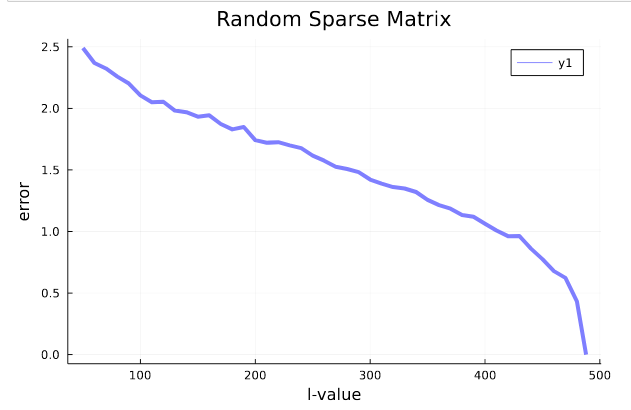
\includegraphics[scale=0.5]{images/4.1_1.png}
	
	\begin{lstlisting}
	A = mmread("data/pde2961.mtx")
	ra = 2961
	xs = collect(100:200:ra)
	if xs[end] != ra
	    xs = [xs ; ra]
	end
	er = zeros(size(xs))
	index = 1
	for i in xs 
	    Q = rrf(A,i)
	    er[index] = opnorm((1.0I - Q*Q')*A)
	    index += 1
	end
	plot(xs, er, xaxis=("l-value"), yaxis="error", line = (0.5, 4, :blue), title="pde2961")
	\end{lstlisting}
	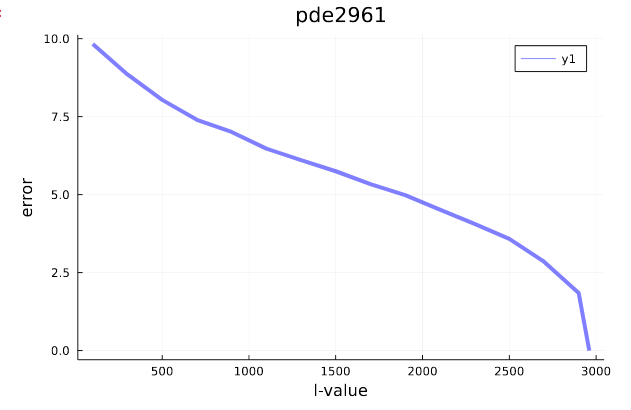
\includegraphics[scale=0.5]{images/4.1_2.png}

	\begin{lstlisting}
	A = mmread("data/eris1176.mtx")
	ra = 774
	xs = collect(74:20:ra)
	if xs[end] != ra
	    xs = [xs ; ra]
	end
	er = zeros(size(xs))
	index = 1
	for i in xs 
	    Q = rrf(A,i)
	    er[index] = opnorm((1.0I - Q*Q')*A)
	    index += 1
	end
	plot(xs, er, xaxis=("l-value"), yaxis="error", line = (0.5, 4, :blue), title="eris1176")
	\end{lstlisting}

	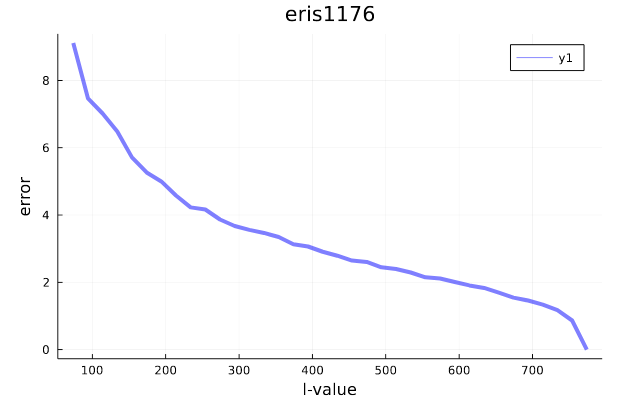
\includegraphics[scale=0.5]{images/4.1_3.png}
	\begin{lstlisting}
	A = mmread("data/lns__511.mtx")
	ra = 391
	xs = collect(41:10:ra)
	if xs[end] != ra
	    xs = [xs ; ra]
	end
	er = zeros(size(xs))
	index = 1
	for i in xs 
	    Q = rrf(A,i)
	    er[index] = opnorm((1.0I - Q*Q')*A)
	    index += 1
	end
	plot(xs, er, xaxis=("l-value"), yaxis="error", line = (0.5, 4, :blue), title="lns__511")
	\end{lstlisting}
	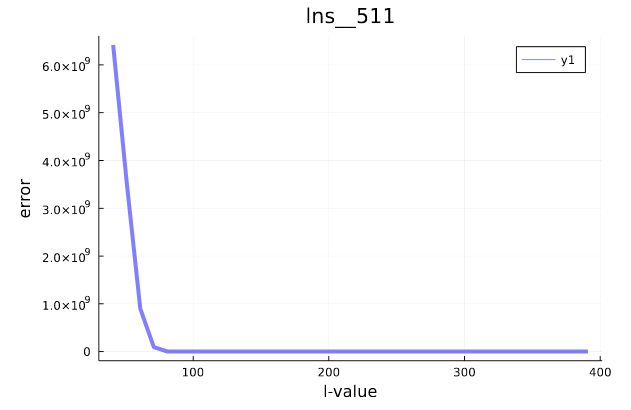
\includegraphics[scale=0.5]{images/4.1_4.png}

	\subsubsection{Test of Algorithm 4.2}
	As detailed in the design and implementation phase algorithm 4.2 returns a matrix $Q$ that approximates the given matrix $A$ up to the error value provided. Below for each test matrix a plot showing that error vs iteration value until algorithm hits the desired error.
	
	\begin{lstlisting}
	A = mmread("data/random_sparse.mtx")
	Q,iterations, errors = arrf(A,0.1, 10, 20);
	mmwrite("data/4.2_random_sparse_output.mtx",sparse(Q))
	plot(iterations, errors, xaxis=("iteration"), yaxis="error", line = (0.5, 4, :blue), title="random_sparse\niteratin vs error")
	\end{lstlisting}
	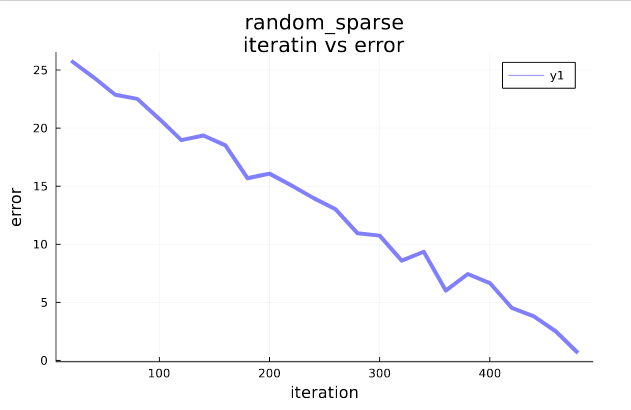
\includegraphics[scale=0.5]{images/4.2_1.png}

	\begin{lstlisting}
	A = mmread("data/pde2961.mtx")
	Q,iterations,errors= arrf(A,0.1, 10, 100);
	mmwrite("data/4.2_pde2961_output.mtx",sparse(Q))
	plot(iterations, errors, xaxis=("iteration"), yaxis="error", line = (0.5, 4, :blue), title="pde2961\niteratin vs error")
	errors = readdlm("data/errors_4.2.1.txt", '\t', Float64, '\n')
	iterations = readdlm("data/iterations_4.2.1.txt", '\t', Int, '\n')
	plot(iterations, errors, xaxis=("iteration"), yaxis="error", line = (0.5, 4, :blue), title="pde2961\niteratin vs error")

	\end{lstlisting}
	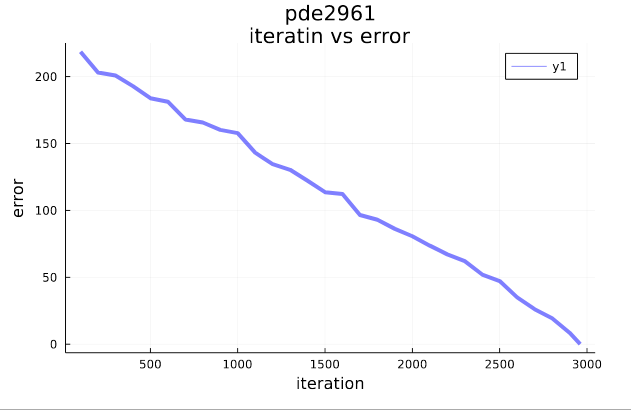
\includegraphics[scale=0.5]{images/4.2_2.png}
	\begin{lstlisting}
	A = mmread("data/eris1176.mtx");
	Q,iterations, errors = arrf(A,0.1,10,20);
	mmwrite("data/4.2_eris1176_output.mtx", sparse(Q))
	plot(iterations, errors, xaxis=("iteration"), yaxis="error", line = (0.5, 4, :blue), title="eris1176\niteratin vs error")


	\end{lstlisting}
	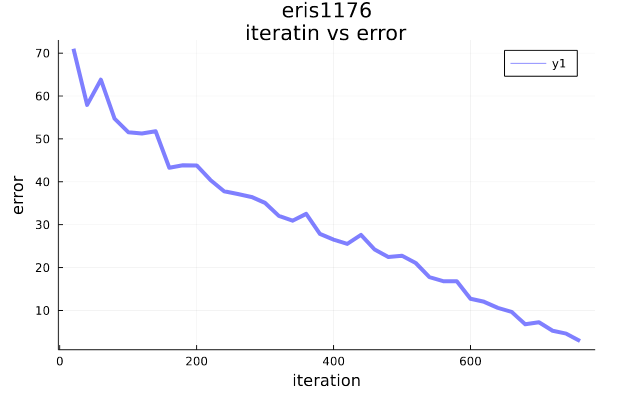
\includegraphics[scale=0.5]{images/4.2_3.png}
	\begin{lstlisting}
	A = mmread("data/lns__511.mtx");
	Q,iterations, errors = arrf(A,1,10,10);
	mmwrite("data/4.2_lns__511_output.mtx", sparse(Q))
	plot(iterations, errors, xaxis=("iteration"), yaxis="error", line = (0.5, 4, :blue), title="lns__511\niteratin vs error")


	\end{lstlisting}
	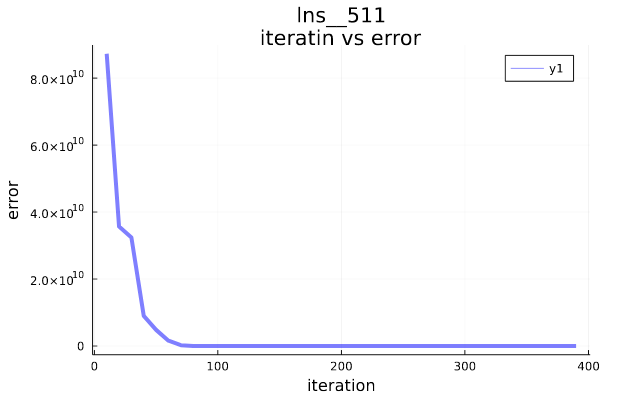
\includegraphics[scale=0.5]{images/4.2_4.png}

	\subsubsection{Test of Algorithm 4.3}
	On this algorithm randomized sampling is applied to the matrix $B = (AA^*)^qA$ instead of $A$. B has same left and right singular vectors ($U$ and $V$) with $A$ but singular values are scaled up and down ($\sigma_j(B) = \sigma_j(A)^{2q+1}$). Hence we expect a quicker range finder algorithm by this change.

	As expected while $q$ is equal zero algorithm works as like algorithm 4.1.

	\begin{lstlisting}
	A = mmread("data/random_sparse.mtx")
	ra = rank(A)
	xs = collect(50:10:ra)
	if xs[end] != ra
	    xs = [xs ; ra]
	end
	er0 = []
	er1 = []
	er3 = []
	er5 = []
	for i in xs 
	    Q0 = rpi(A,i,0)
	    append!(er0,opnorm((1.0I - Q0*Q0')*A))
	end
	plot(xs, er0, xaxis=("l-value"), yaxis="error", line = (0.5, 4, :blue), title="random_sparse\nl-error", label="q=0")
	
	for i in xs 
	        Q1 = rpi(A,i,1)
	        append!(er1,opnorm((1.0I - Q1*Q1')*A))
	end
	plot!(xs, er1, xaxis=("l-value"), yaxis="error", line = (0.5, 4, :yellow), label="q=1")
	
	for i in xs 
	    Q3 = rpi(A,i,1)
	    append!(er3,opnorm((1.0I - Q3*Q3')*A))
	end
	plot!(xs, er3, xaxis=("l-value"), yaxis="error", line = (0.5, 4, :red),label="q=3")
	
	for i in xs 
	    Q5 = rpi(A,i,1)
	    append!(er5,opnorm((1.0I - Q5*Q5')*A))
	end
	plot!(xs, er5, xaxis=("l-value"), yaxis="error", line = (0.5, 4, :green), label="q=5")
	\end{lstlisting}
	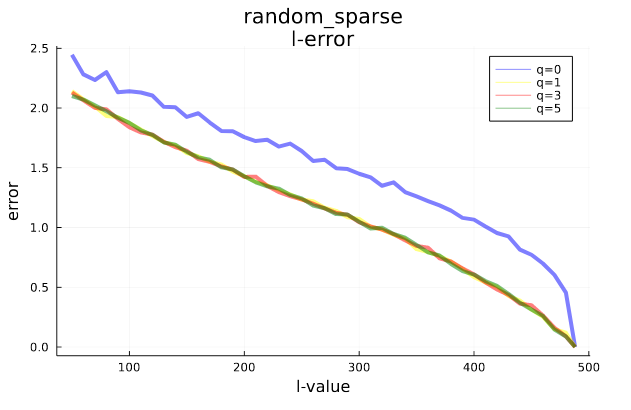
\includegraphics[scale=0.5]{images/4.3_1.png}

	\begin{lstlisting}
	A = mmread("data/pde2961.mtx")
	ra = 2961
	xs = collect(100:200:ra)
	if xs[end] != ra
	    xs = [xs ; ra]
	end
	er0 = []
	er1 = []
	er3 = []
	er5 = []
	for i in xs 
	    Q0 = rpi(A,i,0)
	    append!(er0,opnorm((1.0I - Q0*Q0')*A))
	end
	plot(xs, er0, xaxis=("l-value"), yaxis="error", line = (0.5, 4, :blue), title="pde2961\nl-error", label="q=0")
	
	for i in xs 
	        Q1 = rpi(A,i,1)
	        append!(er1,opnorm((1.0I - Q1*Q1')*A))
	end
	plot!(xs, er1, xaxis=("l-value"), yaxis="error", line = (0.5, 4, :yellow), label="q=1")
	
	for i in xs 
	    Q3 = rpi(A,i,1)
	    append!(er3,opnorm((1.0I - Q3*Q3')*A))
	end
	plot!(xs, er3, xaxis=("l-value"), yaxis="error", line = (0.5, 4, :red),label="q=3")
	
	for i in xs 
	    Q5 = rpi(A,i,1)
	    append!(er5,opnorm((1.0I - Q5*Q5')*A))
	end
	plot!(xs, er5, xaxis=("l-value"), yaxis="error", line = (0.5, 4, :green), label="q=5")
	\end{lstlisting}
	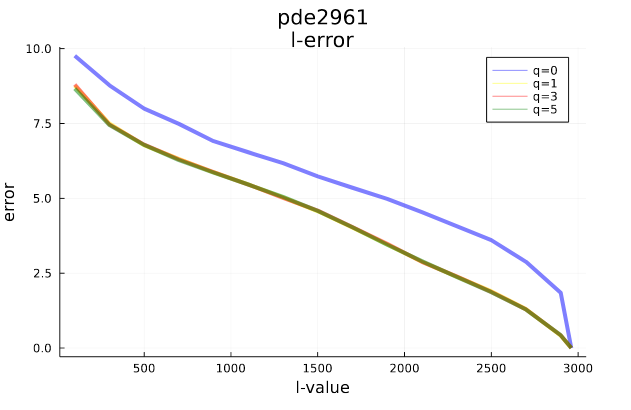
\includegraphics[scale=0.5]{images/4.3_2.png}
	\begin{lstlisting}
	A = mmread("data/eris1176.mtx")
	ra = 774
	xs = collect(74:20:ra)
	if xs[end] != ra
	    xs = [xs ; ra]
	end
	er0 = []
	er1 = []
	er3 = []
	er5 = []
	for i in xs 
	    Q0 = rpi(A,i,0)
	    append!(er0,opnorm((1.0I - Q0*Q0')*A))
	end
	plot(xs, er0, xaxis=("l-value"), yaxis="error", line = (0.5, 4, :blue), title="eris1176\nl-error", label="q=0")
	
	for i in xs 
	        Q1 = rpi(A,i,1)
	        append!(er1,opnorm((1.0I - Q1*Q1')*A))
	end
	plot!(xs, er1, xaxis=("l-value"), yaxis="error", line = (0.5, 4, :yellow), label="q=1")
	
	for i in xs 
	    Q3 = rpi(A,i,1)
	    append!(er3,opnorm((1.0I - Q3*Q3')*A))
	end
	plot!(xs, er3, xaxis=("l-value"), yaxis="error", line = (0.5, 4, :red),label="q=3")
	
	for i in xs 
	    Q5 = rpi(A,i,1)
	    append!(er5,opnorm((1.0I - Q5*Q5')*A))
	end
	plot!(xs, er5, xaxis=("l-value"), yaxis="error", line = (0.5, 4, :green), label="q=5")
	\end{lstlisting}

	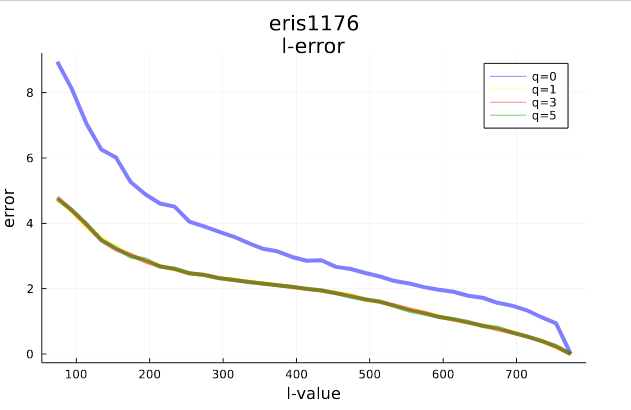
\includegraphics[scale=0.5]{images/4.3_3.png}
	\begin{lstlisting}
	A = mmread("data/lns__511.mtx")
	ra = 391
	xs = collect(41:10:ra)
	if xs[end] != ra
	    xs = [xs ; ra]
	end
	er0 = []
	er1 = []
	er3 = []
	er5 = []
	for i in xs 
	    Q0 = rpi(A,i,0)
	    append!(er0,opnorm((1.0I - Q0*Q0')*A))
	end
	plot(xs, er0, xaxis=("l-value"), yaxis="error", line = (0.5, 4, :blue), title="lns__511\nl-error", label="q=0")
	
	for i in xs 
	        Q1 = rpi(A,i,1)
	        append!(er1,opnorm((1.0I - Q1*Q1')*A))
	end
	plot!(xs, er1, xaxis=("l-value"), yaxis="error", line = (0.5, 4, :yellow), label="q=1")
	
	for i in xs 
	    Q3 = rpi(A,i,1)
	    append!(er3,opnorm((1.0I - Q3*Q3')*A))
	end
	plot!(xs, er3, xaxis=("l-value"), yaxis="error", line = (0.5, 4, :red),label="q=3")
	
	for i in xs 
	    Q5 = rpi(A,i,1)
	    append!(er5,opnorm((1.0I - Q5*Q5')*A))
	end
	plot!(xs, er5, xaxis=("l-value"), yaxis="error", line = (0.5, 4, :green), label="q=5")

	\end{lstlisting}
	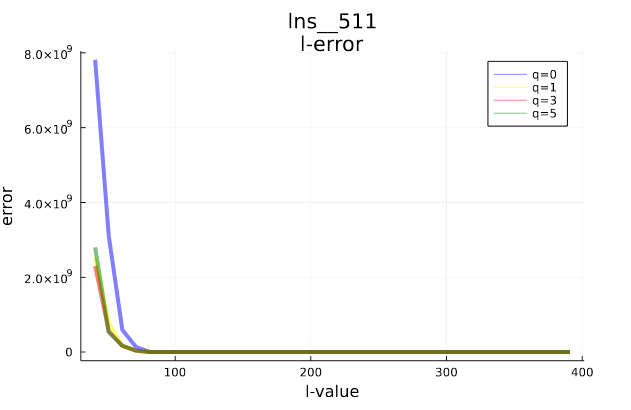
\includegraphics[scale=0.5]{images/4.3_4.png}

	\subsubsection{Algorithm 4.5}
	In this section randomized range finder algorithm 4.1 is presented in comparison with fast randomized range finding algorithm for all the four test matrices.

	\begin{lstlisting}
	A = mmread("data/random_sparse.mtx")
	ra = rank(A)
	xs = collect(50:10:ra)
	if xs[end] != ra
	    xs = [xs ; ra]
	end
	er = zeros(size(xs))
	index = 1
	for i in xs 
	    Q = frrf(A,i)
	    er[index] = opnorm((1.0I - Q*Q')*A)
	    index += 1
	end
	
	p1 = plot(xs, er, xaxis=("l-value"), yaxis="error", line = (0.5, 4, :blue), title="Random Matrix\nFRRF\nl-error")
	
	er = zeros(size(xs))
	index = 1
	for i in xs 
	    Q = rrf(A,i)
	    er[index] = opnorm((1.0I - Q*Q')*A)
	    index += 1
	end
	p2 = plot(xs, er, xaxis=("l-value"), yaxis="error", line = (0.5, 4, :blue), title="Random Matrix\nRRF\nl-error")
	
	plot!(p1,p2)
	\end{lstlisting}
	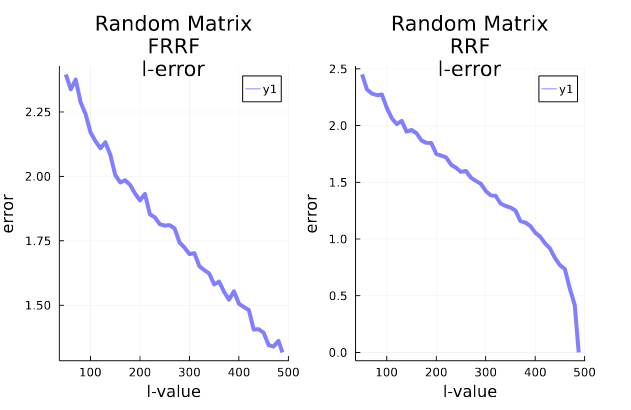
\includegraphics[scale=0.5]{images/4.5_1.png}

	\begin{lstlisting}
	A = mmread("data/pde2961.mtx")
	# @show rank(A) yields rank of A is 2961
	ra = 2961
	xs = collect(100:200:ra)
	if xs[end] != ra
	    xs = [xs ; ra]
	end
	er = zeros(size(xs))
	index = 1
	for i in xs 
	    Q = frrf(A,i)
	    er[index] = opnorm((1.0I - Q*Q')*A)
	    index += 1
	end
	p1 = plot(xs, er, xaxis=("l-value"), yaxis="error", line = (0.5, 4, :blue), title="pde2961\nFRRF\nl-error")
	
	er = zeros(size(xs))
	index = 1
	for i in xs 
	    Q = rrf(A,i)
	    er[index] = opnorm((1.0I - Q*Q')*A)
	    index += 1
	end
	p2 = plot(xs, er, xaxis=("l-value"), yaxis="error", line = (0.5, 4, :blue), title="pde2961\nRRF\nl-error")
	
	plot!(p1,p2)
	\end{lstlisting}
	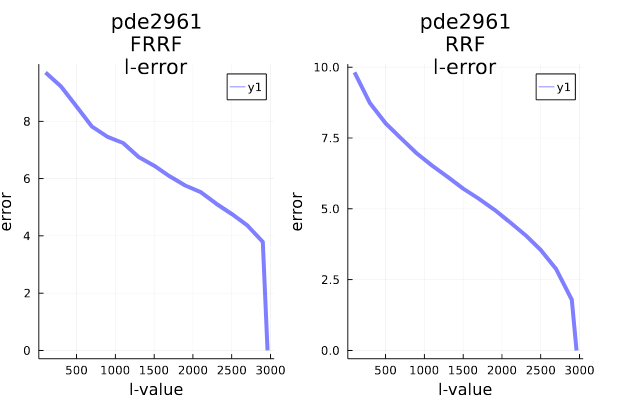
\includegraphics[scale=0.5]{images/4.5_2.png}

	\begin{lstlisting}
	A = mmread("data/eris1176.mtx")
	ra = 774
	xs = collect(74:20:ra)
	if xs[end] != ra
	    xs = [xs ; ra]
	end
	er = zeros(size(xs))
	index = 1
	for i in xs 
	    Q = frrf(A,i)
	    er[index] = opnorm((1.0I - Q*Q')*A)
	    index += 1
	end
	p1 = plot(xs, er, xaxis=("l-value"), yaxis="error", line = (0.5, 4, :blue), title="eris1176\nFRRF\nl-error")
	
	er = zeros(size(xs))
	index = 1
	for i in xs 
	    Q = rrf(A,i)
	    er[index] = opnorm((1.0I - Q*Q')*A)
	    index += 1
	end
	p2 = plot(xs, er, xaxis=("l-value"), yaxis="error", line = (0.5, 4, :blue), title="eris1176\nRRF\nl-error")
	
	plot!(p1,p2)
	\end{lstlisting}
	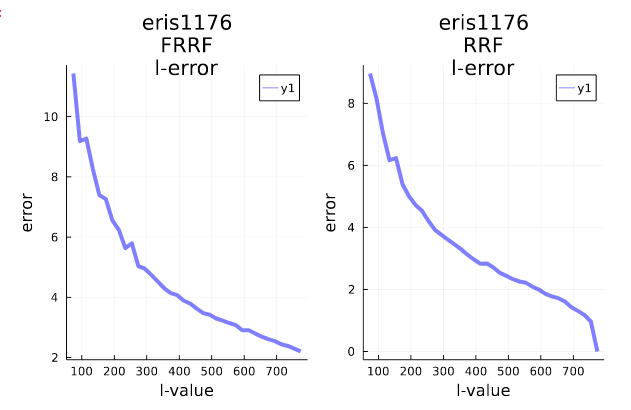
\includegraphics[scale=0.5]{images/4.5_3.png}

	\begin{lstlisting}
	A = mmread("data/lns__511.mtx")
	ra = 391
	xs = collect(41:10:ra)
	if xs[end] != ra
	    xs = [xs ; ra]
	end
	er = zeros(size(xs))
	index = 1
	for i in xs 
	    Q = frrf(A,i)
	    er[index] = opnorm((1.0I - Q*Q')*A)
	    index += 1
	end
	p1 = plot(xs, er, xaxis=("l-value"), yaxis="error", line = (0.5, 4, :blue), title="lns__511\nFRRF\nl-error")
	
	er = zeros(size(xs))
	index = 1
	for i in xs 
	    Q = rrf(A,i)
	    er[index] = opnorm((1.0I - Q*Q')*A)
	    index += 1
	end
	p2 = plot(xs, er, xaxis=("l-value"), yaxis="error", line = (0.5, 4, :blue), title="lns__511\nRRF\nl-error")
	
	plot!(p1,p2)
	\end{lstlisting}
	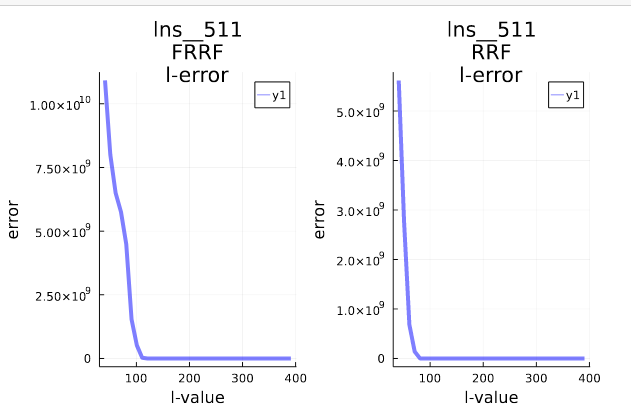
\includegraphics[scale=0.5]{images/4.5_4.png}

	\section{Conclusion}
		In this practice period...
\end{document}





































